\documentclass[12pt,a4paper]{article}
\usepackage{amsmath, amssymb, amsthm}
\usepackage[utf8]{inputenc}
\usepackage[T1]{fontenc}
\usepackage{geometry}
\usepackage{booktabs}
\usepackage{array}
\usepackage{xcolor}
\usepackage{tikz}
\usepackage[most]{tcolorbox}
\usetikzlibrary{arrows.meta, calc}
\geometry{margin=2.5cm}

% ---- Theorem environments ----
\newtheorem{theorem}{Theorem}[section]
\newtheorem{corollary}[theorem]{Corollary}
\newtheorem{lemma}[theorem]{Lemma}
\newtheorem{proposition}[theorem]{Proposition}
\theoremstyle{definition}
\newtheorem{definition}[theorem]{Definition}
\newtheorem{example}[theorem]{Example}
\theoremstyle{remark}
\newtheorem{remark}[theorem]{Remark}
\newtheorem{warning}[theorem]{Warning}

% ---- Convenience macros ----
\newcommand{\R}{\mathbb{R}}
\newcommand{\xbar}{\bar{x}}
\newcommand{\abar}{\bar{a}}
\newcommand{\grad}{\nabla}
\newcommand{\pd}[2]{\dfrac{\partial #1}{\partial #2}}

\title{\textbf{Infinitesimal Calculus 2}\\
\large Master Theorems \& Reference Sheet\\[4pt]
\normalsize Course 21152, HIT --- Prof.\ Anatoly Golberg}
\date{Updated: 2026-03-27}

\begin{document}
\maketitle
\tableofcontents
\newpage

%==============================================================
\section{Improper Integrals (Lecture 1)}
%==============================================================

\begin{definition}[Improper integrals]
\begin{itemize}
  \item \textbf{Type I} (infinite limit):
    $\displaystyle\int_a^{\infty} f(x)\,dx = \lim_{b\to\infty}\int_a^b f(x)\,dx$.
  \item \textbf{Type II} (unbounded integrand at endpoint $b$):
    $\displaystyle\int_a^b f(x)\,dx = \lim_{\varepsilon\to 0^+}\int_a^{b-\varepsilon} f(x)\,dx$.
\end{itemize}
The integral \emph{converges} if the limit exists and is finite; otherwise it \emph{diverges}.
\end{definition}

\subsection*{Reference integrals (p-test)}

\begin{center}
\begin{tabular}{lll}
\toprule
Integral & Converges when & Diverges when \\
\midrule
$\displaystyle\int_1^{\infty}\frac{dx}{x^p}$ & $p>1$ & $p\le 1$ \\[10pt]
$\displaystyle\int_0^{1}\frac{dx}{x^p}$ & $p<1$ & $p\ge 1$ \\
\bottomrule
\end{tabular}
\end{center}

\subsection*{Convergence tests (for $f\ge 0$)}

\begin{theorem}[Comparison Test]
Suppose $0\le f(x)\le g(x)$ for all large $x$.
\begin{itemize}
  \item If $\int g$ converges, then $\int f$ converges.
  \item If $\int f$ diverges, then $\int g$ diverges.
\end{itemize}
\textit{When to use:} When you can bound $f$ from above/below by a known integral.
\end{theorem}

\begin{theorem}[Limit Comparison Test]
Let $f,g\ge 0$ and $\displaystyle L = \lim_{x\to\infty}\frac{f(x)}{g(x)}\in(0,\infty)$.
Then $\int_a^{\infty}f$ and $\int_a^{\infty}g$ have the same convergence behaviour.
\textit{When to use:} When $f\sim C\cdot g$ asymptotically.
\end{theorem}

\begin{remark}[Asymptotic equivalences near $0$]
As $\alpha\to 0$:
\[
  \frac{\sin\alpha}{\alpha}\to 1,\qquad
  \frac{e^{\alpha}-1}{\alpha}\to 1,\qquad
  \frac{\ln(1+\alpha)}{\alpha}\to 1.
\]
\textbf{Strategy}: Near a problematic point, replace each factor by its asymptotic equivalent, then compare with a $p$-integral.
\end{remark}

%==============================================================
\section{Topology of $\R^n$ (Lectures 1 \& 3)}
%==============================================================

\begin{definition}[Euclidean space $\R^n$]
$\R^n$ consists of vectors $\xbar=(x_1,\dots,x_n)$ with the \textbf{Euclidean norm}
\[
  \|\xbar\|_2 = \sqrt{x_1^2+\cdots+x_n^2}.
\]
Other common norms: $\|\xbar\|_1=\sum|x_i|$, $\|\xbar\|_\infty=\max_i|x_i|$.
\end{definition}

\begin{definition}[Norm axioms]
$\|\cdot\|:\R^n\to\R^+$ is a norm if:
\begin{enumerate}
  \item $\|\xbar\|=0 \iff \xbar=0$,
  \item $\|\alpha\xbar\|=|\alpha|\,\|\xbar\|$,
  \item $\|\xbar+\bar{y}\|\le\|\xbar\|+\|\bar{y}\|$ \quad (triangle inequality).
\end{enumerate}
\end{definition}

\begin{theorem}[Cauchy--Schwarz Inequality]
\[
  \left(\sum_{i=1}^n |x_i y_i|\right)^2 \;\le\; \left(\sum_{i=1}^n x_i^2\right)\left(\sum_{i=1}^n y_i^2\right).
\]
\textit{Proof idea}: Define $P(t)=\sum(t|x_i|-|y_i|)^2\ge 0$; this quadratic in $t$ has non-positive discriminant.
\end{theorem}

\begin{definition}[Metric / distance]
$d(\xbar,\bar{y})=\|\xbar-\bar{y}\|$.  It satisfies: $d\ge 0$; $d=0\iff\xbar=\bar{y}$; symmetry; triangle inequality.
\end{definition}

\subsection*{Topological notions}

\begin{definition}[Open ball]
$B(\abar,r)=\{\xbar:\|\xbar-\abar\|<r\}$.
\end{definition}

Let $E\subseteq\R^n$.
\begin{center}
\renewcommand{\arraystretch}{1.4}
\begin{tabular}{lll}
\toprule
Type & Condition & Notation\\
\midrule
Interior point & $\exists\,r>0:\,B(\abar,r)\subseteq E$ & $\operatorname{Int}E$\\
Exterior point & $\exists\,r>0:\,B(\abar,r)\cap E=\emptyset$ & $\operatorname{Ext}E$\\
Boundary point & Every $B(\abar,r)$ meets both $E$ and $\R^n\setminus E$ & $\partial E$\\
\bottomrule
\end{tabular}
\end{center}

\begin{definition}[Open, closed, bounded, compact]
\begin{itemize}
  \item \textbf{Open}: $E=\operatorname{Int}E$ (every point is interior).
  \item \textbf{Closed}: $\partial E\subseteq E$ (equivalently: $\R^n\setminus E$ is open).
  \item \textbf{Bounded}: $E\subseteq B(\abar,r)$ for some ball.
  \item \textbf{Compact}: closed $+$ bounded.
\end{itemize}
\end{definition}

\begin{theorem}[Weierstrass --- existence of extrema]
If $f$ is continuous on a compact set $E\subseteq\R^n$, then:
\begin{enumerate}
  \item $f$ is \emph{bounded} on $E$.
  \item $f$ attains its supremum $M=\sup_E f$ and infimum $m=\inf_E f$ on $E$.
\end{enumerate}
\end{theorem}

%==============================================================
\section{Multivariable Functions --- Limits \& Continuity (Lectures 2--3)}
%==============================================================

\begin{definition}[Limit --- Heine definition]
$\displaystyle\lim_{\xbar\to\abar}f(\xbar)=L$ if for every sequence
$\xbar^{(m)}\to\abar$ (with $\xbar^{(m)}\ne\abar$), we have $f(\xbar^{(m)})\to L$.
\end{definition}

\begin{definition}[Limit --- Cauchy / $\varepsilon$-$\delta$ definition]
$\displaystyle\lim_{\xbar\to\abar}f(\xbar)=L$ if
\[
  \forall\varepsilon>0\;\exists\,\delta>0:\quad 0<\|\xbar-\abar\|<\delta\;\Longrightarrow\;|f(\xbar)-L|<\varepsilon.
\]
\end{definition}

\begin{theorem}
The Heine and Cauchy definitions are equivalent.
\end{theorem}

\subsection*{Techniques for evaluating limits}

\begin{remark}[Two-path test for non-existence]
To prove $\lim f$ \textbf{does not exist}: find two paths to $\abar$ giving different limit values.
\end{remark}

\begin{remark}[Polar coordinates]
Set $x=\rho\cos\theta$, $y=\rho\sin\theta$.  If $f(\rho,\theta)\to L$ as $\rho\to 0$ \emph{uniformly in $\theta$}, then $\lim_{(x,y)\to(0,0)}f=L$.

\textbf{Pitfall}: If the expression in polar still depends on $\theta$ without vanishing, the limit may not exist; fall back to the two-path method.
\end{remark}

\begin{remark}[Squeeze theorem]
If $|f(\xbar)-L|\le g(\xbar)$ and $g(\xbar)\to 0$, then $f(\xbar)\to L$.
\end{remark}

\subsection*{Key examples}

\begin{center}
\renewcommand{\arraystretch}{1.5}
\begin{tabular}{lll}
\toprule
Function at $(0,0)$ & Result & Method \\
\midrule
$\dfrac{xy}{x^2+y^2}$ & DNE & Paths $y=0$ (value 0), $y=x$ (value $\tfrac12$) \\[8pt]
$\dfrac{xy^2}{x^2+y^2}$ & $0$ & Polar: $\rho\cos\theta\sin^2\theta\to 0$; squeeze $\le|y|$ \\[8pt]
$\dfrac{xy^2}{x^2+y^4}$ & DNE & Paths $y=0$ (value 0), $x=y^2$ (value $\tfrac12$) \\[8pt]
$\dfrac{x^2y^2(x^2+y^2)}{x^4+y^4}$ & $0$ & Polar, bound $\cos^4\!\theta+\sin^4\!\theta\ge\tfrac12$ \\[8pt]
$\dfrac{\sin(x-y)}{x-y}$ & DNE & Not defined on $y=x$; no punctured nbhd \\
\bottomrule
\end{tabular}
\end{center}

\begin{remark}[Useful bound in polar]
\[
  \cos^4\!\theta + \sin^4\!\theta = 1 - 2\cos^2\!\theta\sin^2\!\theta = 1 - \tfrac12\sin^2\!2\theta \;\ge\; \frac{1}{2}.
\]
\end{remark}

\begin{definition}[Continuity]
$f$ is \textbf{continuous} at $\abar$ if $\displaystyle\lim_{\xbar\to\abar}f(\xbar)=f(\abar)$.
Equivalently: $\Delta f(\abar)=f(\abar+\Delta\xbar)-f(\abar)\to 0$ as $\Delta\xbar\to 0$.
\end{definition}

%==============================================================
\section{Partial Derivatives \& Differentiability (Lecture 4)}
%==============================================================

\subsection*{Partial derivatives}

\begin{definition}[First-order partial derivatives]
For $z=f(x,y)$ at $(x_0,y_0)$:
\[
  f'_x(x_0,y_0) = \lim_{\Delta x\to 0}\frac{f(x_0+\Delta x,\,y_0)-f(x_0,y_0)}{\Delta x},
  \qquad
  f'_y(x_0,y_0) = \lim_{\Delta y\to 0}\frac{f(x_0,\,y_0+\Delta y)-f(x_0,y_0)}{\Delta y}.
\]
\textit{Computationally}: differentiate w.r.t.\ $x$ treating $y$ constant (and vice versa).
\end{definition}

\subsection*{Differentiability}

\begin{definition}[Differentiability]
$f(x,y)$ is \textbf{differentiable} at $(x_0,y_0)$ if the total increment satisfies
\[
  \Delta f = A\,\Delta x + B\,\Delta y + \alpha\,\Delta x + \beta\,\Delta y,
\]
where $\alpha,\beta\to 0$ as $(\Delta x,\Delta y)\to(0,0)$.
The expression $A\,\Delta x+B\,\Delta y$ is the \textbf{total differential} $df$.
Equivalently:
\[
  \lim_{\Delta\rho\to 0}\frac{\varepsilon}{\Delta\rho} = 0,
  \qquad \varepsilon = \Delta f - f_x\,\Delta x - f_y\,\Delta y,\quad \Delta\rho=\sqrt{\Delta x^2+\Delta y^2}.
\]
\end{definition}

\begin{remark}[Intuition for $\varepsilon/R\to 0$]
$\Delta f$ is the \emph{actual} change in $f$; $df = f_x\,\Delta x+f_y\,\Delta y$ is the \emph{linear approximation} of that change.
Their difference $\varepsilon$ is the error. Differentiability asks:
\begin{center}
\emph{Does the error $\varepsilon$ shrink to zero faster than the distance $R$ moved?}
\end{center}
A small absolute error is not enough — $\varepsilon$ must become \emph{negligible relative to $R$} (i.e.\ $\varepsilon = o(R)$).
Geometrically: the tangent plane is a \emph{good} local approximation of $f$, not just any approximation.
\end{remark}

\subsection*{Hierarchy of properties}

\begin{theorem}[Thm 1: Differentiable $\Rightarrow$ Continuous]
If $f$ is differentiable at $(x_0,y_0)$, it is continuous there.
(\emph{Converse is false.})
\end{theorem}

\begin{theorem}[Thm 2: Differentiable $\Rightarrow$ partial derivatives exist]
If $f$ is differentiable at $(x_0,y_0)$, then $f_x$ and $f_y$ exist there, and $A=f_x$, $B=f_y$.
(\emph{Converse is false.})
\end{theorem}

\begin{theorem}[Thm 3 --- Sufficient condition for differentiability]
If $f_x$ and $f_y$ exist in a neighbourhood of $(x_0,y_0)$ and are \emph{continuous} there,
then $f$ is differentiable at $(x_0,y_0)$.
(\emph{Converse is false.})
\end{theorem}

\begin{center}
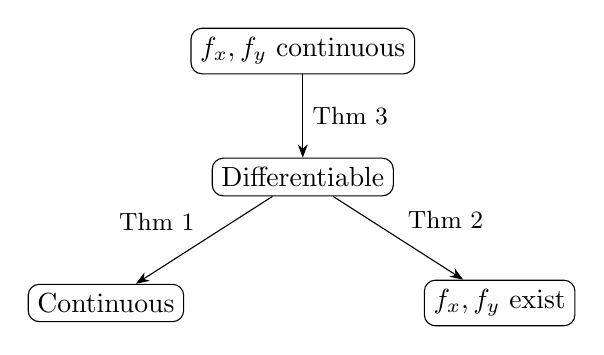
\begin{tikzpicture}[>=Stealth]
  \node[draw, rounded corners] (A) at (0,0)  {$f_x,f_y$ continuous};
  \node[draw, rounded corners] (B) at (0,-1.6) {Differentiable};
  \node[draw, rounded corners] (C) at (-2.5,-3.2) {Continuous};
  \node[draw, rounded corners] (D) at (2.5,-3.2) {$f_x,f_y$ exist};
  \draw[->] (A) -- node[right]{\small Thm 3} (B);
  \draw[->] (B) -- node[above left]{\small Thm 1} (C);
  \draw[->] (B) -- node[above right]{\small Thm 2} (D);
\end{tikzpicture}
\end{center}

\begin{warning}
None of the reverse implications hold in general!
\end{warning}

\subsection*{Counterexamples (know these!)}

\begin{center}
\renewcommand{\arraystretch}{1.4}
\begin{tabular}{llll}
\toprule
Function & At $(0,0)$ & Holds & Fails \\
\midrule
$f=\dfrac{xy}{x^2+y^2},\;f(0,0)=0$ & $(0,0)$ & $f_x=f_y=0$ exist & Continuous, differentiable \\[8pt]
$f=\dfrac{x^2 y}{x^4+y^2},\;f(0,0)=0$ & $(0,0)$ & $f_x=f_y=0$ exist & Continuous, differentiable \\[8pt]
$f=|x|+\sqrt[3]{y^2}$ & $(0,0)$ & Continuous & Partial derivatives \\[8pt]
$f=(x^2+y^2)\sin\!\dfrac{1}{x^2+y^2},\;f(0,0)=0$ & $(0,0)$ & Differentiable ($df=0$) & $f_x,f_y$ continuous \\
\bottomrule
\end{tabular}
\end{center}

\begin{tcolorbox}[title={How to check differentiability at $(x_0,y_0)$}, colback=blue!5, colframe=blue!40!black]
\textbf{Step 1 — Quick pass (sufficient condition):}
If $f_x$ and $f_y$ both exist and are \emph{continuous} near the point $\Rightarrow$ differentiable. Done.

\medskip
\textbf{Step 2 — Must use definition (piecewise / suspicious point):}
\begin{enumerate}
  \item Compute $f_x(x_0,y_0)$ and $f_y(x_0,y_0)$ from the \emph{limit definition} (not formula).
  \item Form the error: $\varepsilon = \Delta f - f_x\,\Delta x - f_y\,\Delta y$.
  \item Check: $\displaystyle\lim_{R\to 0}\frac{\varepsilon}{R} = 0$ where $R=\sqrt{\Delta x^2+\Delta y^2}$.
  \item \textit{Trick:} substitute polar coords $\Delta x = r\cos\theta$, $\Delta y=r\sin\theta$, $R=r$.
        If after simplification $r$ cancels and a $\theta$-dependent expression remains $\Rightarrow$ limit does not exist $\Rightarrow$ \textbf{not differentiable}.
\end{enumerate}

\medskip
\textbf{Step 3 — Consequences (check the chain):}
\[
  f_x,f_y \text{ continuous} \;\Rightarrow\; \text{differentiable} \;\Rightarrow\; \text{continuous} \;\Rightarrow\; \text{partials exist}
\]
None of the reverse implications hold.

\medskip
\textbf{Warning — directional derivatives:}
$D_{\bar{u}}f = \nabla f\cdot\hat{u}$ is valid \emph{only if $f$ is differentiable}.
At suspicious points, always use the definition:
$D_{\hat{u}}f(x_0,y_0) = \lim_{t\to 0}\dfrac{f(x_0+tu_1,\,y_0+tu_2)}{t}$.
\end{tcolorbox}

\subsection*{Total differential \& linear approximation}

\begin{definition}[Total differential]
\[
  df = f_x\,dx + f_y\,dy \quad (\text{or } f_x\,\Delta x + f_y\,\Delta y \text{ for finite increments}).
\]
\end{definition}

\begin{remark}[Linear approximation]
\[
  f(x_0+\Delta x,\,y_0+\Delta y)\;\approx\; f(x_0,y_0)+f_x(x_0,y_0)\,\Delta x+f_y(x_0,y_0)\,\Delta y.
\]
Use near a known point $(x_0,y_0)$ where $f$ is differentiable.
\end{remark}

\begin{remark}[Tangent plane to $z=f(x,y)$]
\[
  z - f(a,b) = f_x(a,b)(x-a) + f_y(a,b)(y-b).
\]
Normal direction: $\bar{n}=(f_x(a,b),\,f_y(a,b),\,-1)$.
\end{remark}

\subsection*{Higher-order partial derivatives}

\begin{definition}
$f_{xx}=\pd{}{x}\!\left(\pd{f}{x}\right)$, $\;f_{xy}=\pd{}{y}\!\left(\pd{f}{x}\right)$, etc.
\end{definition}

\begin{theorem}[Schwarz / Clairaut --- mixed partial derivatives]
If $f_{xy}$ and $f_{yx}$ are both \emph{continuous} in a neighbourhood of $(x_0,y_0)$, then
\[
  f_{xy}(x_0,y_0)=f_{yx}(x_0,y_0).
\]
\end{theorem}

%==============================================================
\section{Directional Derivative \& Gradient (Week 3)}
%==============================================================

\begin{definition}[Directional derivative]
For a unit vector $\bar{u}$:
\[
  D_{\bar{u}}f(\abar) = \lim_{t\to 0}\frac{f(\abar+t\bar{u})-f(\abar)}{t}.
\]
If $f$ is differentiable: $D_{\bar{u}}f = \grad f\cdot\bar{u}$.
\end{definition}

\begin{definition}[Gradient]
\[
  \grad f = \left(\pd{f}{x},\pd{f}{y}\right)
  \quad\text{(or with $\pd{f}{z}$ in $\R^3$).}
\]
\end{definition}

\begin{theorem}[Properties of the gradient]
\begin{itemize}
  \item $\|\grad f\|$ = maximum rate of change of $f$.
  \item The direction of $\grad f$ gives the direction of steepest ascent.
  \item $\grad f \perp$ level curves (level surfaces).
\end{itemize}
\end{theorem}

\begin{remark}[Tangent plane to level surface $F(x,y,z)=C$]
\[
  F_x(P)(x-x_0)+F_y(P)(y-y_0)+F_z(P)(z-z_0)=0, \quad P=(x_0,y_0,z_0).
\]
\end{remark}

%==============================================================
\section{Chain Rule (Weeks 2--4)}
%==============================================================

\begin{theorem}[Chain rule --- one parameter]
If $z=f(x,y)$, $x=x(t)$, $y=y(t)$:
\[
  \frac{dz}{dt} = \pd{f}{x}\frac{dx}{dt}+\pd{f}{y}\frac{dy}{dt}.
\]
\end{theorem}

\begin{theorem}[Chain rule --- two parameters]
If $z=f(x,y)$, $x=x(u,v)$, $y=y(u,v)$:
\[
  \pd{z}{u} = \pd{f}{x}\pd{x}{u}+\pd{f}{y}\pd{y}{u},
  \qquad
  \pd{z}{v} = \pd{f}{x}\pd{x}{v}+\pd{f}{y}\pd{y}{v}.
\]
\end{theorem}

\begin{remark}[Polar chain rule]
$w=f(x,y)$ with $x=r\cos t$, $y=r\sin t$:
\[
  \frac{1}{r}\pd{w}{t} = -f_x\sin t + f_y\cos t.
\]
\end{remark}

\subsection*{Fundamental Theorem of Calculus --- applied to partial derivatives}

\begin{theorem}[FTC with variable limits]
If $f(t)$ is continuous, define $F(x,y) = \displaystyle\int_x^y f(t)\,dt$. Then:
\[
  \pd{F}{y} = f(y), \qquad \pd{F}{x} = -f(x).
\]
More generally, if both limits depend on parameters:
\[
  \pd{}{u}\int_{a(u)}^{b(u)} f(t)\,dt = f(b(u))\cdot b'(u) - f(a(u))\cdot a'(u).
\]
\end{theorem}

\begin{remark}[Why the minus sign on the lower limit]
Split at any fixed point $c$:
\[
  \int_x^y f(t)\,dt = \int_c^y f(t)\,dt - \int_c^x f(t)\,dt.
\]
Differentiating the second term w.r.t.\ $x$ gives $-f(x)$.
\end{remark}

\begin{remark}[Direct usage --- do NOT integrate]
When asked to differentiate $z = \int_x^y f(t)\,dt$, apply FTC immediately.
There is no need (and often no way) to find an antiderivative first.

\textbf{Classic trap}: $f(t) = e^{t^2}$ has \emph{no elementary antiderivative}.
Integration by parts will not close.  Apply FTC directly:
\[
  \pd{z}{y} = e^{y^2}, \qquad \pd{z}{x} = -e^{x^2}.
\]
\end{remark}

%==============================================================
\section{Taylor Polynomial \& Local Extrema (Week 4)}
%==============================================================

\begin{theorem}[Taylor polynomial of order 2]
\[
  f(a+h,b+k) = f(a,b) + \bigl[f_x h + f_y k\bigr]
  + \tfrac{1}{2}\bigl[f_{xx}h^2 + 2f_{xy}hk + f_{yy}k^2\bigr] + \cdots
\]
\end{theorem}

\begin{theorem}[Second derivative test for local extrema]
Let $(a,b)$ be a critical point ($\grad f=0$). Define the \textbf{Hessian determinant}:
\[
  D = f_{xx}f_{yy} - (f_{xy})^2.
\]
\begin{center}
\begin{tabular}{cll}
\toprule
$D$ & $f_{xx}$ & Conclusion \\
\midrule
$D>0$ & $f_{xx}>0$ & Local \textbf{minimum} \\
$D>0$ & $f_{xx}<0$ & Local \textbf{maximum} \\
$D<0$ & --- & \textbf{Saddle point} \\
$D=0$ & --- & \textbf{Inconclusive} \\
\bottomrule
\end{tabular}
\end{center}
\end{theorem}

\begin{theorem}[Sylvester's criterion ($n$ variables)]
For the Hessian matrix $H$ with leading principal minors $\Delta_1,\Delta_2,\dots,\Delta_n$:
\begin{itemize}
  \item \textbf{Positive definite} (local min): all $\Delta_k>0$.
  \item \textbf{Negative definite} (local max): signs alternate $\Delta_1<0,\Delta_2>0,\Delta_3<0,\dots$
  \item Otherwise: indefinite (saddle) or inconclusive.
\end{itemize}
\end{theorem}

\begin{remark}[Positive definite quadratic form in 2 variables]
$Q(h,k)=ah^2+2bhk+ck^2$:
\begin{itemize}
  \item Positive definite $\iff a>0$ and $ac-b^2>0$.
  \item Negative definite $\iff a<0$ and $ac-b^2>0$.
\end{itemize}
\end{remark}

%==============================================================
\section{Implicit Functions \& Lagrange Multipliers (Week 5)}
%==============================================================

\begin{theorem}[Implicit Function Theorem (2 variables)]
If $F(x,y)=0$, $F$ is $C^1$, $F(x_0,y_0)=0$, and $F_y(x_0,y_0)\ne 0$, then near $(x_0,y_0)$
there is a unique function $y=\varphi(x)$ with $F(x,\varphi(x))=0$ and
\[
  \varphi'(x) = -\frac{F_x}{F_y}.
\]
\end{theorem}

\begin{theorem}[Implicit Function Theorem (3 variables)]
For $F(x,y,z)=0$ with $F_z\ne 0$:
\[
  \pd{z}{x} = -\frac{F_x}{F_z},\qquad \pd{z}{y} = -\frac{F_y}{F_z}.
\]
\end{theorem}

\begin{theorem}[Lagrange Multipliers]
To optimize $f(x,y)$ subject to $g(x,y)=0$, solve:
\[
  \grad f = \lambda\,\grad g, \quad g(x,y)=0.
\]
i.e.\ $f_x=\lambda g_x$,\; $f_y=\lambda g_y$,\; $g=0$.

For \textbf{two constraints} $g_1=0,\,g_2=0$:
$\grad f = \lambda_1\grad g_1+\lambda_2\grad g_2$.
\end{theorem}

\begin{remark}[Global extrema on compact domain]
\begin{enumerate}
  \item Find interior critical points ($\grad f=0$).
  \item Find boundary extrema (parametrize boundary or use Lagrange multipliers).
  \item Compare all candidate values; largest = global max, smallest = global min.
\end{enumerate}
\end{remark}

%==============================================================
\section{Double Integrals (Weeks 6--7)}
%==============================================================

\begin{definition}[Double integral properties]
$\iint_D f\,dA$: linearity, additivity over regions, monotonicity ($f\ge 0\Rightarrow\iint f\ge 0$).
\end{definition}

\begin{theorem}[Fubini's Theorem]
If $f$ is continuous on $D$:
\begin{itemize}
  \item \textbf{Type I}: $D=\{a\le x\le b,\;g_1(x)\le y\le g_2(x)\}$
    \[\iint_D f\,dA = \int_a^b\!\!\int_{g_1(x)}^{g_2(x)} f(x,y)\,dy\,dx.\]
  \item \textbf{Type II}: $D=\{c\le y\le d,\;h_1(y)\le x\le h_2(y)\}$
    \[\iint_D f\,dA = \int_c^d\!\!\int_{h_1(y)}^{h_2(y)} f(x,y)\,dx\,dy.\]
\end{itemize}
\end{theorem}

\begin{theorem}[Change of variables in double integrals]
\[
  \iint_D f(x,y)\,dA = \iint_{D^*} f(x(u,v),y(u,v))\,|J|\,du\,dv,
\]
where $J = \dfrac{\partial(x,y)}{\partial(u,v)} = x_u y_v - x_v y_u$ is the \textbf{Jacobian}.
\end{theorem}

\begin{remark}[Polar coordinates: $x=r\cos\theta,\;y=r\sin\theta$]
$|J|=r$, so:
\[
  \iint_D f(x,y)\,dx\,dy = \iint_{D^*} f(r\cos\theta,\,r\sin\theta)\cdot r\,dr\,d\theta.
\]
\textit{Use when}: $x^2+y^2$ appears or the domain is circular/sector-shaped.
\end{remark}

%==============================================================
\section{Line Integrals (Weeks 7--8)}
%==============================================================

\begin{definition}[Line integral of Type I --- scalar / arc length]
\[
  \int_C f\,ds = \int_a^b f(\mathbf{r}(t))\,|\mathbf{r}'(t)|\,dt,
  \quad |\mathbf{r}'(t)|=\sqrt{x'(t)^2+y'(t)^2}.
\]
If $f=1$: gives the arc length of $C$.
\end{definition}

\begin{definition}[Line integral of Type II --- vector field / work]
\[
  \int_C P\,dx+Q\,dy = \int_a^b \bigl[P(\mathbf{r}(t))x'(t)+Q(\mathbf{r}(t))y'(t)\bigr]\,dt.
\]
\textit{Note}: reversing the orientation negates the integral.
\end{definition}

%==============================================================
\section{Green's Theorem \& Conservative Fields (Week 8)}
%==============================================================

\begin{theorem}[Green's Theorem]
Let $C$ be a positively oriented (CCW), simple, closed curve bounding $D$:
\[
  \oint_C P\,dx+Q\,dy = \iint_D\left(\pd{Q}{x}-\pd{P}{y}\right)dA.
\]
\textit{Applications}: area of $D = \oint_C x\,dy = -\oint_C y\,dx = \tfrac12\oint_C(x\,dy-y\,dx)$.
\end{theorem}

\begin{theorem}[Conservative (gradient) fields --- equivalent conditions]
For $\mathbf{F}=(P,Q)$ on a simply connected domain, the following are equivalent:
\begin{enumerate}
  \item $\mathbf{F}=\grad\varphi$ for some potential $\varphi$ (\emph{conservative}).
  \item $\int_C\mathbf{F}\cdot d\mathbf{r}$ is path-independent.
  \item $\oint_C\mathbf{F}\cdot d\mathbf{r}=0$ for every closed curve.
  \item $\displaystyle\pd{P}{y}=\pd{Q}{x}$ \quad (\emph{necessary}; \emph{sufficient} on simply connected domain).
\end{enumerate}
If conservative: $\displaystyle\int_C\mathbf{F}\cdot d\mathbf{r}=\varphi(\text{end})-\varphi(\text{start})$.
\end{theorem}

\begin{remark}[Finding the potential]
\begin{enumerate}
  \item Integrate: $\varphi=\int P\,dx + g(y)$.
  \item Differentiate: $\varphi_y=Q$, solve for $g(y)$.
\end{enumerate}
\end{remark}

%==============================================================
\section{Triple Integrals (Weeks 8--9)}
%==============================================================

\begin{theorem}[Fubini for triple integrals]
$\iiint_B f\,dV = \int\!\!\int\!\!\int f(x,y,z)\,dx\,dy\,dz$ (iterate in any order over rectangular box).
For general domains: set up variable bounds from a sketch.
\end{theorem}

\begin{remark}[Cylindrical coordinates: $x=r\cos\theta,\;y=r\sin\theta,\;z=z$]
$|J|=r$:
\[
  \iiint f\,dV = \iiint f(r\cos\theta,r\sin\theta,z)\cdot r\,dr\,d\theta\,dz.
\]
\textit{Use when}: $x^2+y^2$ appears (circular symmetry in $xy$-plane).
\end{remark}

\begin{remark}[Spherical coordinates: $x=\rho\sin\varphi\cos\theta,\;y=\rho\sin\varphi\sin\theta,\;z=\rho\cos\varphi$]
$|J|=\rho^2\sin\varphi$, with $\rho\ge 0$, $0\le\varphi\le\pi$, $0\le\theta\le 2\pi$:
\[
  \iiint f\,dV = \iiint f(\cdots)\cdot\rho^2\sin\varphi\,d\rho\,d\varphi\,d\theta.
\]
\textit{Use when}: $x^2+y^2+z^2$ appears (spherical symmetry).
\end{remark}

%==============================================================
\section{Surface Integrals (Week 10)}
%==============================================================

\begin{definition}[Surface integral of Type I --- scalar]
\[
  \iint_S f\,dS = \iint_D f(\mathbf{r}(u,v))\,|\mathbf{r}_u\times\mathbf{r}_v|\,du\,dv.
\]
For $z=g(x,y)$: $dS=\sqrt{1+g_x^2+g_y^2}\,dx\,dy$.
\end{definition}

\begin{definition}[Surface integral of Type II --- flux]
\[
  \iint_S \mathbf{F}\cdot d\mathbf{S} = \iint_D \mathbf{F}\cdot(\mathbf{r}_u\times\mathbf{r}_v)\,du\,dv.
\]
\end{definition}

\begin{definition}[Divergence and curl]
\[
  \operatorname{div}\mathbf{F} = \nabla\cdot\mathbf{F} = \pd{P}{x}+\pd{Q}{y}+\pd{R}{z},
\]
\[
  \operatorname{curl}\mathbf{F} = \nabla\times\mathbf{F} =
  \begin{vmatrix}\mathbf{i}&\mathbf{j}&\mathbf{k}\\\pd{}{x}&\pd{}{y}&\pd{}{z}\\P&Q&R\end{vmatrix}.
\]
\end{definition}

%==============================================================
\section{Gauss \& Stokes Theorems (Week 11)}
%==============================================================

\begin{theorem}[Divergence Theorem (Gauss)]
\[
  \iint_{\partial V} \mathbf{F}\cdot d\mathbf{S} = \iiint_V (\nabla\cdot\mathbf{F})\,dV.
\]
Converts flux through a closed surface to a volume integral of the divergence.
\end{theorem}

\begin{theorem}[Stokes' Theorem]
\[
  \oint_C \mathbf{F}\cdot d\mathbf{r} = \iint_S (\nabla\times\mathbf{F})\cdot d\mathbf{S}.
\]
\textit{Note}: Green's theorem is the 2D special case.
\end{theorem}

%==============================================================
\section{Differential Forms \& Generalized Stokes (Week 12)}
%==============================================================

\begin{definition}[Differential forms]
\begin{itemize}
  \item \textbf{0-form}: function $f$.
  \item \textbf{1-form}: $\omega = P\,dx+Q\,dy+R\,dz$.
  \item \textbf{2-form}: $\omega = P\,dy\wedge dz + Q\,dz\wedge dx + R\,dx\wedge dy$.
  \item \textbf{3-form}: $\omega = f\,dx\wedge dy\wedge dz$.
\end{itemize}
\end{definition}

\begin{definition}[Exterior derivative]
$d$ maps $k$-forms to $(k{+}1)$-forms:
$d(\text{0-form})=\text{gradient}$, $d(\text{1-form})=\text{curl}$, $d(\text{2-form})=\text{divergence}$.

\textbf{Key property}: $d(d\omega)=0$.
\end{definition}

\begin{theorem}[Generalized Stokes' Theorem]
\[
  \int_{\partial\Omega}\omega = \int_\Omega d\omega.
\]
\begin{center}
\begin{tabular}{ll}
\toprule
Theorem & Dimension \\
\midrule
Fundamental Theorem of Calculus & 1D \\
Green's Theorem & 2D \\
Classical Stokes' Theorem & 3D (curve $\leftrightarrow$ surface) \\
Gauss / Divergence Theorem & 3D (surface $\leftrightarrow$ volume) \\
\bottomrule
\end{tabular}
\end{center}
\end{theorem}

%==============================================================
\section*{Problem-Solving Strategy Cheat Sheet}
\addcontentsline{toc}{section}{Problem-Solving Strategy Cheat Sheet}
%==============================================================

\begin{enumerate}
  \item \textbf{Improper integral convergence?} Identify type (I or II). Find asymptotic equivalent near the singular point. Compare with $p$-integral.
  \item \textbf{Multivariable limit?} Try two paths first (to disprove). If paths agree, try polar/squeeze (to prove).
  \item \textbf{Continuity at $(0,0)$?} Check $\lim f = f(0,0)$ using polar or squeeze.
  \item \textbf{Differentiability at $(0,0)$?} (1) Compute $f_x(0,0)$, $f_y(0,0)$ from definition. (2) Verify $\lim_{\Delta\rho\to 0}[\Delta f - f_x\Delta x - f_y\Delta y]/\Delta\rho = 0$. \emph{Or}: if $f_x,f_y$ are continuous $\Rightarrow$ differentiable (Thm 3).
  \item \textbf{Tangent plane?} For $z=f$: use gradient. For $F=C$: use $\grad F$.
  \item \textbf{Chain rule?} Draw dependency tree; multiply partial derivatives along each path and sum.
  \item \textbf{Local extrema?} Solve $\grad f=0$, apply Hessian/Sylvester.
  \item \textbf{Constrained optimization?} Lagrange multipliers.
  \item \textbf{Global extrema on compact domain?} Critical points inside + boundary extrema; compare all values.
  \item \textbf{Double integral?} Sketch region; choose order of integration; use polar if $x^2+y^2$ appears.
  \item \textbf{Triple integral?} Cylindrical if $x^2+y^2$; spherical if $x^2+y^2+z^2$.
  \item \textbf{Line integral?} Type I: parametrize + $|\mathbf{r}'|$. Type II: check conservative first $\to$ potential or Green's.
  \item \textbf{Surface integral / flux?} Parametrize + cross product. Closed surface $\to$ Gauss.
  \item \textbf{Closed curve in 3D?} Consider Stokes' theorem.
\end{enumerate}

\end{document}
